\documentclass{article} % For LaTeX2e
\usepackage[legalpaper, margin=0.5in]{geometry}
\usepackage{amsmath}
\usepackage{amsfonts,dsfont}
\usepackage{amssymb}
\usepackage[ruled,vlined]{algorithm2e}

\usepackage{graphicx}
\usepackage{caption}
\usepackage{subcaption}
\usepackage{xcolor}

\DeclareMathOperator*{\argmin}{arg\,min}
\DeclareMathOperator*{\argmax}{arg\,max}

\begin{document}

\section{Compact Description For Anomalies}

Providing explanations for anomalies is important and some recent work (among others) can be found in \cite{macha:2017}. We illustrate a different and yet very simple approach when AAD is used with \textit{Isolation Forest}.

The Isolation Forest version of AAD works by partitioning the space into smaller subspaces and weights each subspace to fit the expert feedback. The end result is: (1) a set of default (unsupervised) anomaly scores for each subspace and, (2) weights for each subspace inferred from feedback. We can generate compact descriptions for the anomalies using this information. The idea is to select some combination of (preferably) the smallest subspaces that \textbf{cover} all \textbf{discovered} anomalies. Therefore, we treat this as an instance of the \emph{set covering} problem. We illustrate this on a toy dataset below.

Assume that there are total $m$ subspaces across all Isolation Forest trees. We represent weights by ${\bf w} \in \mathbb{R}^m$, and the corresponding unsupervised anomaly scores by ${\bf d} \in \mathbb{R}^m$.

Now, the final anomaly scores for the \textbf{subspaces} (not instances), after incorporating feedback, is ${\bf a} = {\bf w} \circ {\bf d} \in \mathbb{R}^m$ where $\circ$ denotes the element wise (\textit{Hadamard}) product.

We sort the scores in ${\bf a}$ in descending order and select (say) $30$ top ranked subspaces. Next, we retain only those subspaces from this set which contain at least one anomaly \textbf{discovered} by the analyst. Let us denote the resulting set of subspaces by $\mathcal{S}$. Further, let $\mathcal{Z}$ be the set of discovered anomalies that belong to one or more subspaces in $\mathcal{S}$, and $|\mathcal{Z}|=n$. (Note that some of the discovered anomalies might not belong to any of the top ranked subspaces we selected.)

Let $|\mathcal{S}|=k$. Denote the \textit{volumes} of the subspaces in $\mathcal{S}$ by the vector ${\bf v} \in \mathbb{R}^k$. Now, assume that a binary vector ${\bf x} \in \{0, 1\}^k$ contains $1$ in locations corresponding to the subspaces in $\mathcal{S}$ which are included in the covering set, and $0$ otherwise. Let ${\bf u}_z \in \{0, 1\}^k$ denote a vector for each anomaly $z \in \mathcal{Z}$ which contains $1$ in all locations corresponding to the subspaces in $\mathcal{S}$ that $z$ belongs to. Let ${\bf U} \in \{0, 1\}^{[n \times k]}$ represent the matrix of all ${\bf u}$s.

The selection of the compact set of subspaces to describe all discovered anomalies can be formulated as:
\begin{align}
& \argmin_{{\bf x} \in \{0, 1\}^k} {\bf x} \cdot {\bf v}^p \label{eqn:opt} \\
\text{s.t.} & {\bf U} \cdot {\bf x} \geq {\bf 1} \nonumber \\
\text{where, } & \text{${\bf 1}$ is the column vector of $n$ 1s, and} \nonumber \\
& \text{$p$ is an integer $\geq 1$ (more below)} \nonumber
\end{align}

The parameter $p$ determines how severely to penalize larger volumes. This is usually $1$. However, a larger value will strongly discourage bigger volume subspaces from being selected.

We apply this idea on a toy data shown in Figure~\ref{fig:dataset}. The compact descriptions are shown in Figure~\ref{fig:compact_rects}.

Note that we have not considered labeled nominals in the optimization objective, but a more sophisticated objective might include them too. For instance, we could add another term in the objective which penalizes whenever a nominal is present in the selected subspace.

A different approach to generate descriptions might train a cost-based decision tree with the labeled anomalies and nominals. Once trained, the extracted rules would correspond to `descriptions'. This approach is possibly more principled because the decision tree splits are [usually] based on information gain or gini-index and are therefore more informative. The downside is that this would be separate from the anomaly detector and therefore it would not offer much insight into the anomaly detector's behavior -- ideally we would like the explanation or description of anomalies to reflect the detector's internals.

\begin{figure}
	\centering
	\begin{subfigure}[b]{0.3\textwidth}
		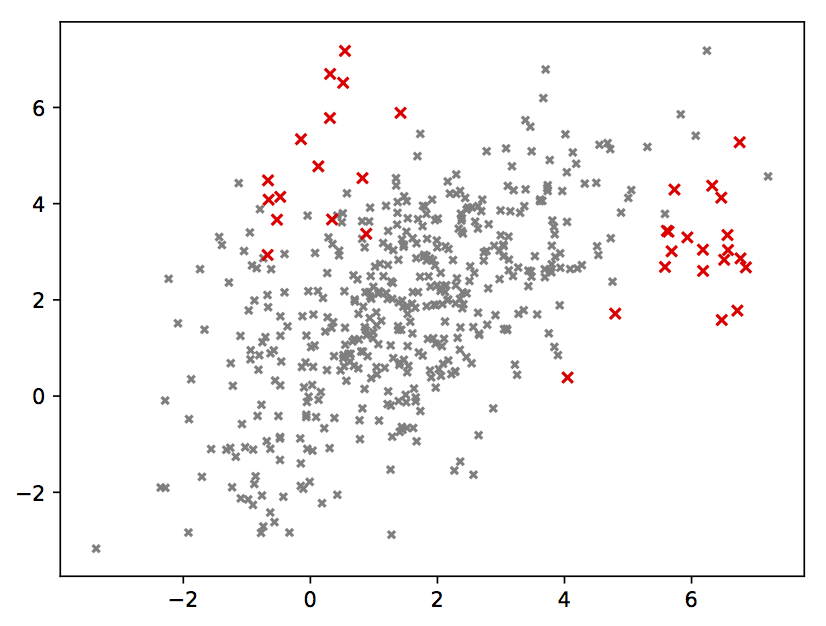
\includegraphics[width=\textwidth]{toy2_dataset}
		\caption{Dataset}
		\label{fig:dataset}
	\end{subfigure}
	~ %add desired spacing between images, e. g. ~, \quad, \qquad, \hfill etc. 
	%(or a blank line to force the subfigure onto a new line)
	\begin{subfigure}[b]{0.3\textwidth}
		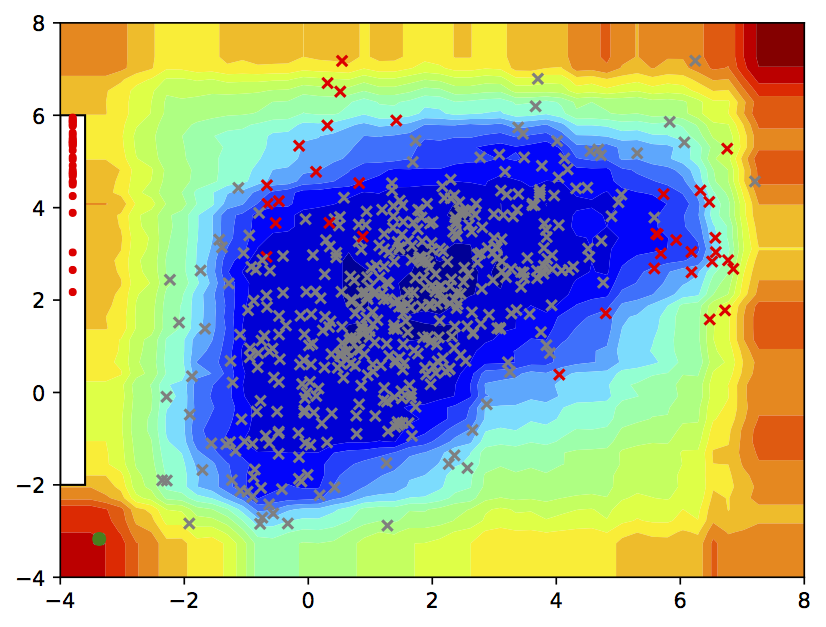
\includegraphics[width=\textwidth]{toy2_iter_00}
		\caption{Initial score contours}
		\label{fig:baseline_contours}
	\end{subfigure}
	~ %add desired spacing between images, e. g. ~, \quad, \qquad, \hfill etc. 
	%(or a blank line to force the subfigure onto a new line)
	\begin{subfigure}[b]{0.3\textwidth}
		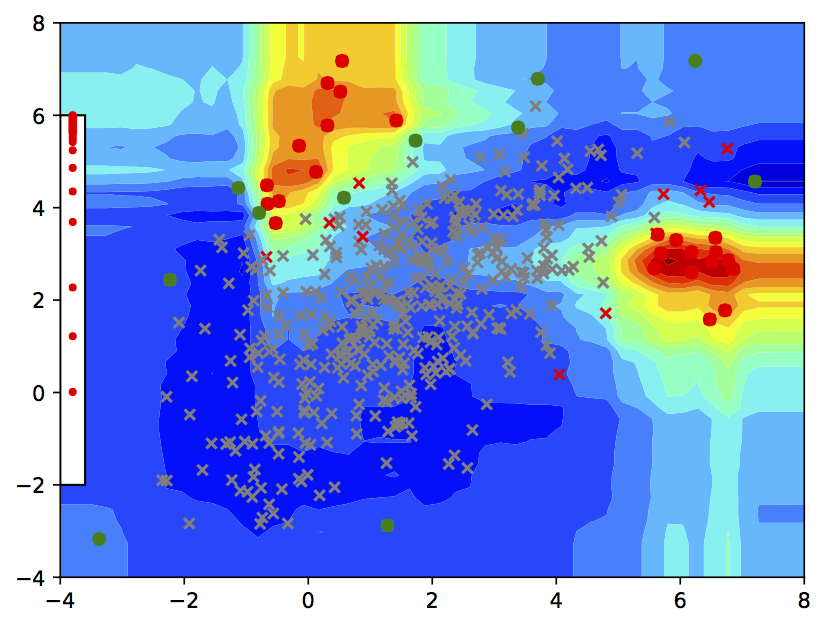
\includegraphics[width=\textwidth]{toy2_iter_34}
		\caption{After 35 feedback}
		\label{fig:contours_35}
	\end{subfigure}
	\caption{Dataset and score contours. Figure~\ref{fig:dataset} shows a synthetic toy dataset. Figure~\ref{fig:baseline_contours} shows the initial Isolation Forest score contours. Figure~\ref{fig:contours_35} shows the score contours after 35 feedback iterations from the Oracle. The red dots are discovered anomalies (true positives). The green dots are discovered nominals (false positives). The red checks are undiscovered anomalies (false negatives).} \label{fig:dataset_and_contours}
\end{figure}

\begin{figure}
	\centering
	\begin{subfigure}[b]{0.3\textwidth}
		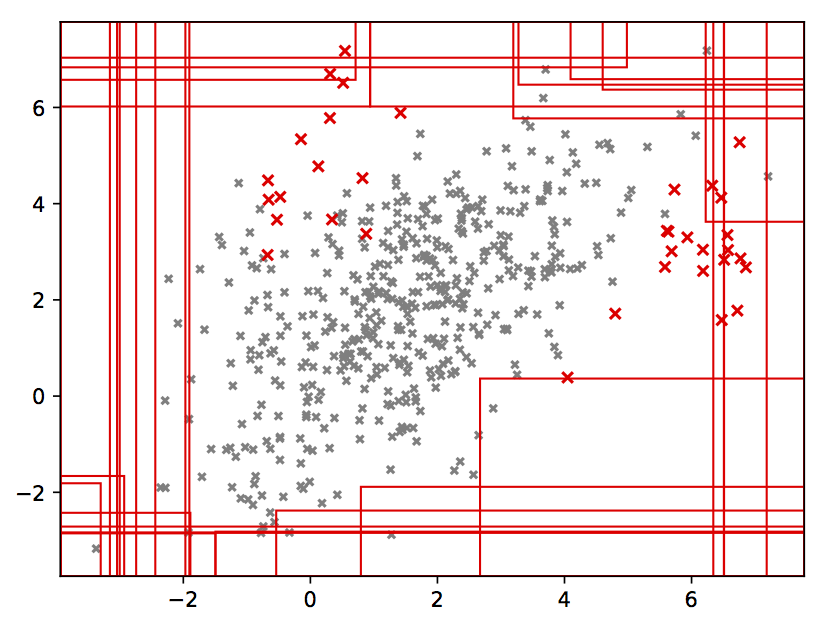
\includegraphics[width=\textwidth]{top_30_anomalous_regions_100_trees_baseline}
		\caption{Baseline}
		\label{fig:baseline_rects}
	\end{subfigure}
	~ %add desired spacing between images, e. g. ~, \quad, \qquad, \hfill etc. 
	%(or a blank line to force the subfigure onto a new line)
	\begin{subfigure}[b]{0.3\textwidth}
		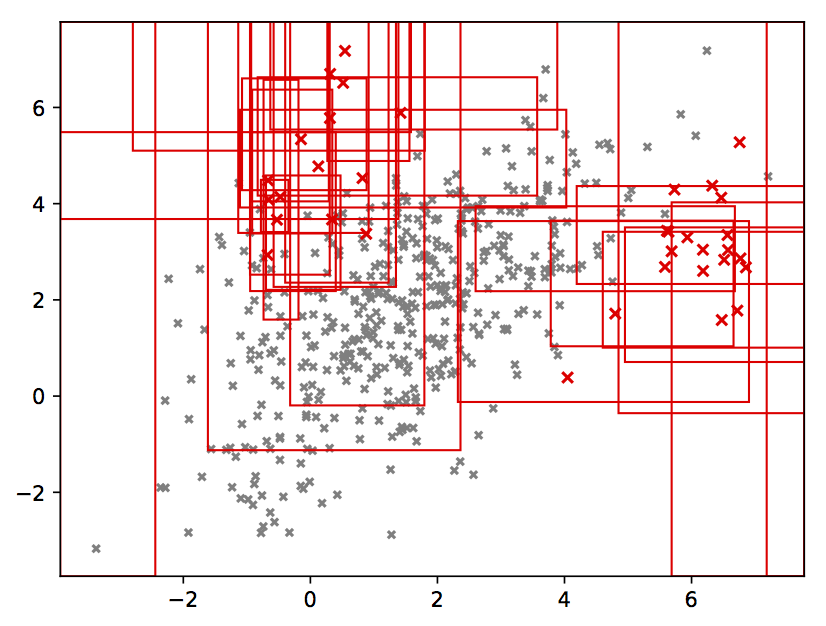
\includegraphics[width=\textwidth]{top_30_anomalous_regions_100_trees_aad}
		\caption{AAD}
		\label{fig:aad_rects}
	\end{subfigure}
	~ %add desired spacing between images, e. g. ~, \quad, \qquad, \hfill etc. 
	%(or a blank line to force the subfigure onto a new line)
	\begin{subfigure}[b]{0.3\textwidth}
		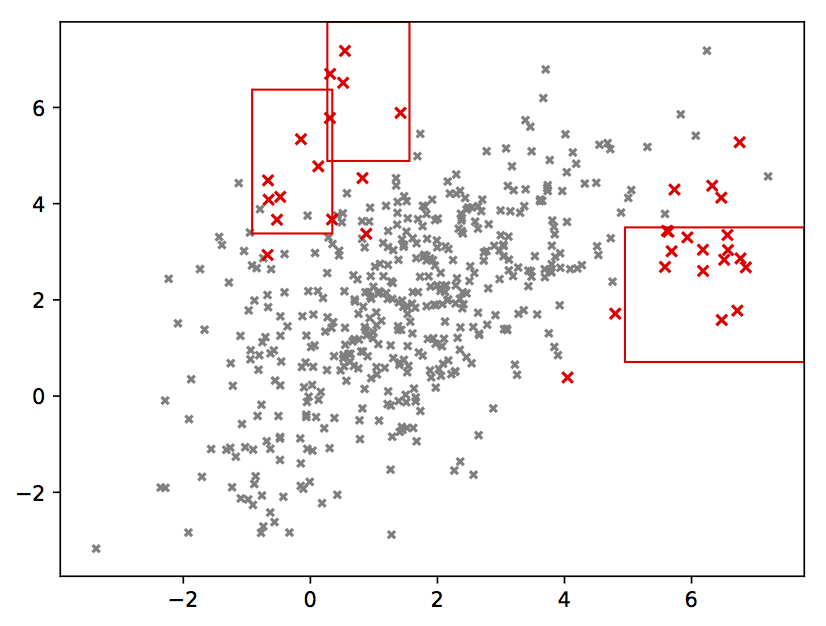
\includegraphics[width=\textwidth]{top_30_anomalous_regions_100_trees_compact}
		\caption{Compact AAD}
		\label{fig:compact_rects}
	\end{subfigure}
	\caption{Top $30$ subspaces ranked by ${\bf w}\circ{\bf d}$. Figure~\ref{fig:baseline_rects} shows the top $30$ most important subspaces (w.r.t their \textit{anomalousness}) without any feedback. We can see that initially, these simply correspond to the exterior regions of the dataset. AAD \textbf{learns the true importance of subspaces} automatically with feedback. For example, after incorporating the labels of $35$ instances, the subspaces around the labeled anomalies have emerged as the most important (Figure~\ref{fig:aad_rects}). Figure~\ref{fig:compact_rects} shows the most compact set of subspaces (for AAD) which cover all labeled anomalies. These are computed with Equation~\ref{eqn:opt}. We might even think of this as a non-parametric clustering. Note that the compact subspaces only cover anomalies that were discovered in the $35$ feedback iterations. Anomalies which were not detected are likely to fall outside these compact subspaces.} \label{fig:rects}
\end{figure}

\section{Querying Diversity}
We can use the anomaly description to diversify our queries when we have the option to query labels for more than one instance per round of feedback. Following is how we go about it:
\begin{enumerate}
	\item Select the top ranked $m$ (say, $m=15$) instances. Denote this set by $\mathcal{C}$ (points in \textcolor{blue}{blue} in Figure~\ref{fig:candidate_regions}).
	\item Next, select the top (say) $5$ most anomalous regions for each instance in $\mathcal{C}$. Let $\mathcal{F}$ be the union of all these regions (rectangles in \textcolor{red}{red} in Figure~\ref{fig:candidate_regions}).
	\item Now, \emph{compactly} describe all instances in $\mathcal{C}$ using the regions in $\mathcal{F}$ (rectangles in \textcolor{red}{red} in Figure~\ref{fig:baseline_queries}).
	\item Now, start with the most anomalous instance, and select one-by-one $k$ (say, $k=5$) instances which have the fewest overlapping regions for querying (points circled in \textcolor{green}{green} in Figures \ref{fig:baseline_queries} and \ref{fig:diverse_queries}).
\end{enumerate}

\begin{figure}
	\centering
	\begin{subfigure}[b]{0.48\textwidth}
		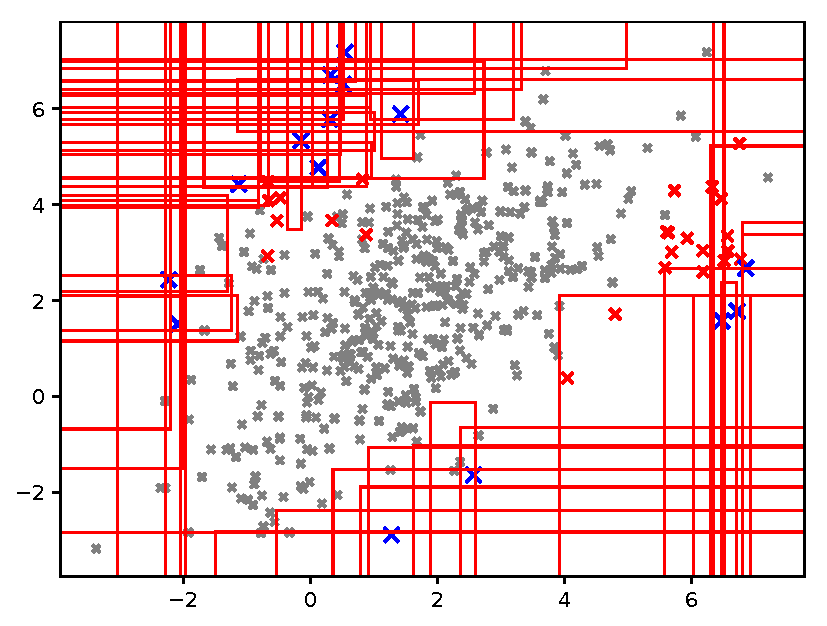
\includegraphics[width=\textwidth]{query_candidate_regions_ntop5_100_trees}
		\caption{Candidate regions and instances}
		\label{fig:candidate_regions}
	\end{subfigure}
	%~ %add desired spacing between images, e. g. ~, \quad, \qquad, \hfill etc. 
	%(or a blank line to force the subfigure onto a new line)
	\begin{subfigure}[b]{0.48\textwidth}
		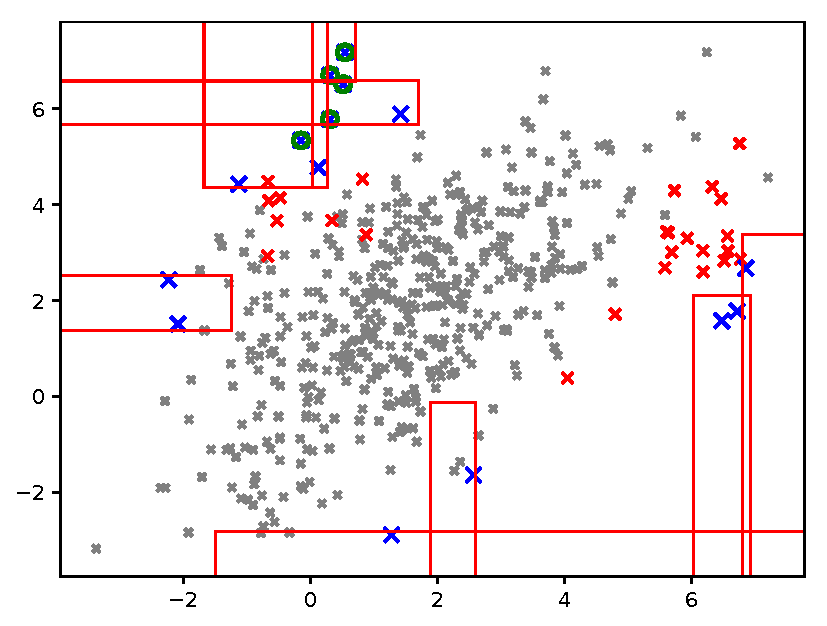
\includegraphics[width=\textwidth]{query_compact_ntop5_100_trees_baseline}
		\caption{Simple select-top query}
		\label{fig:baseline_queries}
	\end{subfigure} \\
    %~
	\begin{subfigure}[b]{0.48\textwidth}
		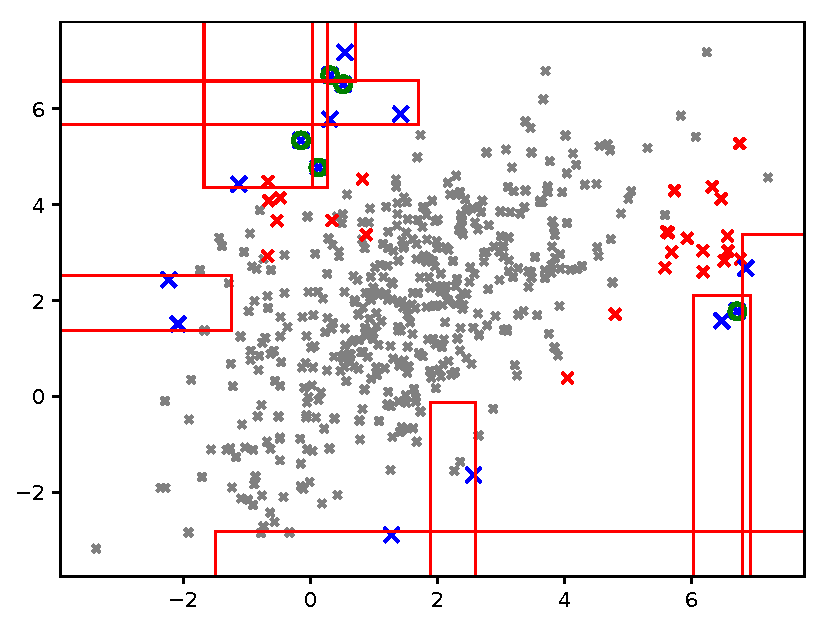
\includegraphics[width=\textwidth]{query_compact_ntop5_100_trees_aad}
		\caption{Select diverse query}
		\label{fig:diverse_queries}
	\end{subfigure}
	\caption{Diverse querying strategy using sub-space descriptions. These figures show the $15$ most anomalous instances (ranked by score) in \textcolor{blue}{blue}. We assume that the true labels are not known for these instances. We find the top $5$ most anomalous regions for each of the $15$ instances and the union of all these regions is shown as the \textcolor{red}{red} rectangles in Figure~\ref{fig:candidate_regions}. Figure~\ref{fig:baseline_queries} and Figure~\ref{fig:diverse_queries} show the regions which compactly contain (describe) the top-ranked instances. The instances circled in \textcolor{green}{green} are the ones selected for querying. The instances (in green) in Figure~\ref{fig:baseline_queries} are merely the top-ranked $5$ instances without taking into account any diversity. Figure~\ref{fig:diverse_queries} shows that when we select instances which have different descriptions (minimum region overlap), they are more diverse.} \label{fig:diverse}
\end{figure}

\subsection{Does the diverse querying strategy help?}
Whatever querying strategy we use, it should ideally not lower the number of anomalies discovered within a budget. For the diverse query strategy, we need to 

\begin{figure}
	\centering
	\begin{subfigure}[b]{0.48\textwidth}
		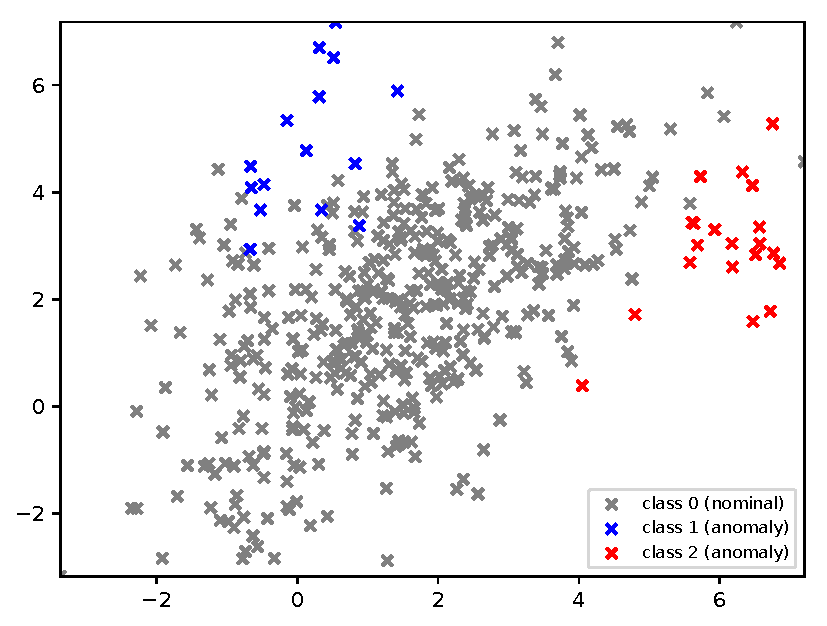
\includegraphics[width=\textwidth]{toy2_processes}
		\caption{Underlying Processes}
		\label{fig:processes}
	\end{subfigure}
	%~ %add desired spacing between images, e. g. ~, \quad, \qquad, \hfill etc. 
	%(or a blank line to force the subfigure onto a new line)
	\begin{subfigure}[b]{0.48\textwidth}
		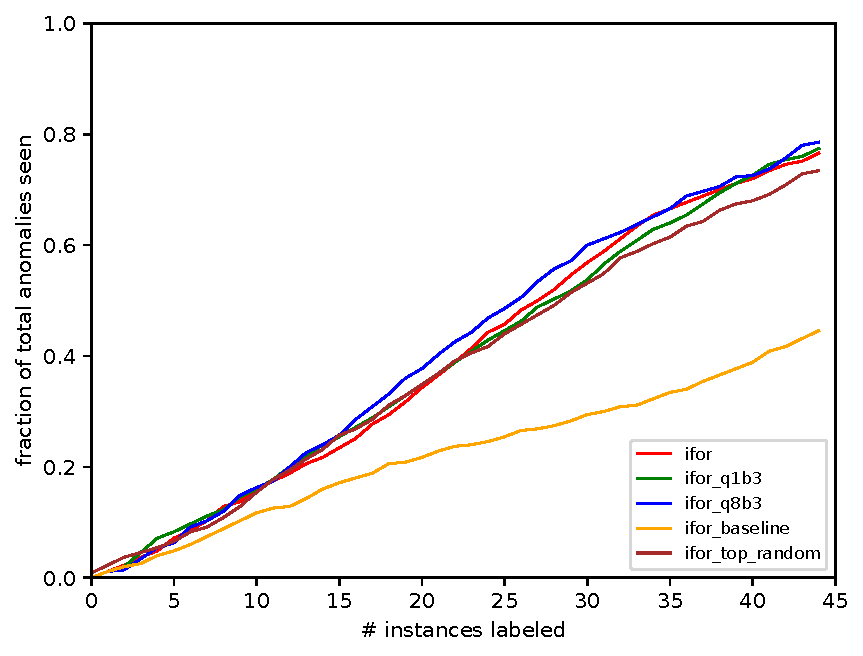
\includegraphics[width=\textwidth]{results_anoms_found_toy2}
		\caption{Anomalies discovered}
		\label{fig:discovery}
	\end{subfigure} \\
	%~
	\begin{subfigure}[b]{0.48\textwidth}
		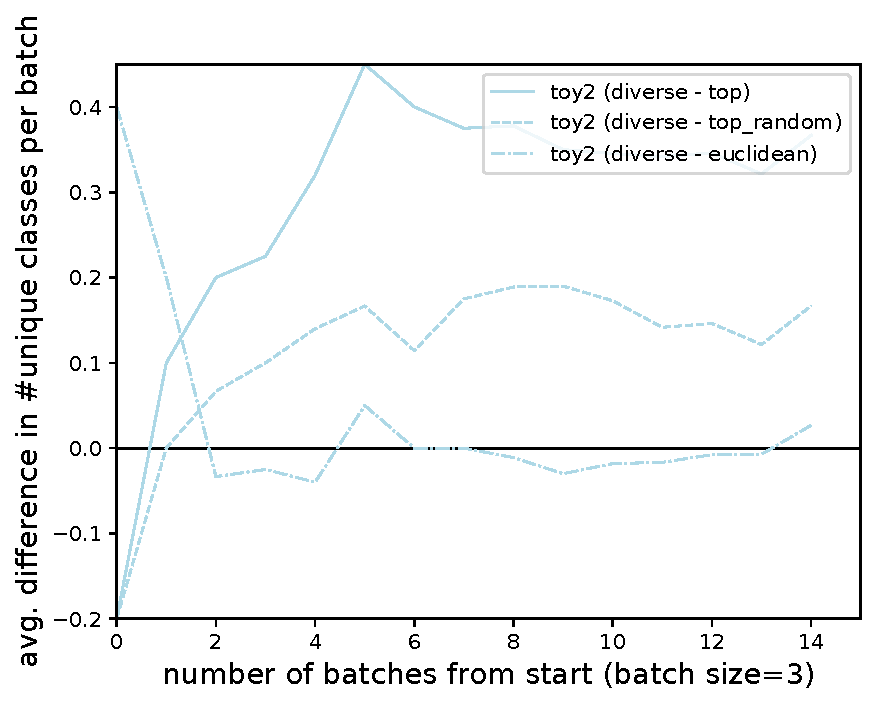
\includegraphics[width=\textwidth]{results_diff_classes_toy2}
		\caption{Difference in class diversity per batch}
		\label{fig:class_diff}
	\end{subfigure}
	\caption{Diversity in the classes shown to an analyst per batch. Here we assume that the data contains \textbf{three} classes which represent three underlying processes (Figure~\ref{fig:processes}). Class $0$ is \emph{nominal}, while classes $1$ and $2$ are \emph{anomalous}. In Figure~\ref{fig:discovery}, we plot the anomaly discovery curves for five Isolation Forest-based algorithms: (a) \textbf{BAL (Adaptive Prior)} -- label only the single most anomalous instance (per iteration), (b) \textbf{ifor\_q1b3} -- label the top three most anomalous instances, (c) \textbf{BAL-D} -- label the top three \textbf{most diverse} instances among the top ten anomalous instances (employing the diversity strategy), (d) \textbf{BAL-E} -- label the top three instances \textbf{farthest in euclidean space} among the top ten anomalous instances, (e) \textbf{Unsupervised Baseline} -- unsupervised Isolation Forest, and (f) \textbf{ifor\_top\_random} -- label three instances selected uniformly at random from the top ten anomalous instances. We see that all algorithms other than the baseline have similar performance, and all active labeling algorithms perform better than the baseline. In Figure~\ref{fig:class_diff}, the solid line \texttt{(diverse - top)} shows the average difference in the number of unique classes shown to the analyst per batch between \textbf{BAL-D} and \textbf{ifor\_q1b3} (these differences are averaged over $10$ runs). The dashed line \texttt{(diverse - top\_random)} in Figure~\ref{fig:class_diff} shows the average difference in the number of unique classes shown to the analyst per batch between \textbf{BAL-D} and \textbf{ifor\_top\_random}. Since both these differences are mostly positive, we conclude that the diversity strategy indeed presents more diverse instances to the analyst to label. Moreover, as seen in Figure~\ref{fig:discovery}, this diversity does not lower the anomaly detection accuracy over a strictly select-top-anomalous query strategy. \textbf{We also see this pattern in most real-world datasets we experimented with.} The dash-dot line \texttt{(diverse - euclidean)} shows the difference between \textbf{BAL-D} and \textbf{BAL-E}. \textbf{BAL-E} is a standard way to find diverse instances. The performance of \textbf{BAL-D} and \textbf{BAL-E} are very similar; however, \textbf{BAL-D} is more user-friendly because it provides descriptions which can characterize multiple anomalies.} \label{fig:diverse_effect}
\end{figure}

\section{Comparison between Isolation Forest, HS Trees, RS Forest}
There are fundamental differences between Isolation Forest and the other two: HS Trees and RS Forest. These differences directly influence the effectiveness of incorporating feedback. Since the depths in HS Trees and RS Forest are fixed and they repeatedly split a dimension, there are $O(2^H)$ subspaces represented by the leaf nodes of these detectors and most are very small in volume. We see this property in Figures \ref{fig:hstrees_rects} and \ref{fig:rsforest_rects}. The implication is that more number of subspaces will be required to generate a compact representation for a set of instances. This also means that feedback at instance level is going to be shared by a much fewer set of instances. In contrast, in Isolation forest (Figure~\ref{fig:iforest_rects}), the depths of leaf nodes are not fixed; they are usually \textbf{much} shallower than in HS Trees and  RS Forest. As a result, the subspaces represented by the leaf nodes are larger and cover more number of instances, thereby requiring fewer subspaces to compactly represent a set of instances. Moreover, this results in feedback being shared by more instances in Isolation Forest. One remedy for HS Trees and RS Forest might be to dynamically determine when to stop splitting based on (maybe) the number of samples at a node. This might be a motivation for future research. My personal opinion right now is to stick to Isolation Forest because of its `nicer' properties.

\begin{figure}
	\centering
	\begin{subfigure}[b]{0.3\textwidth}
		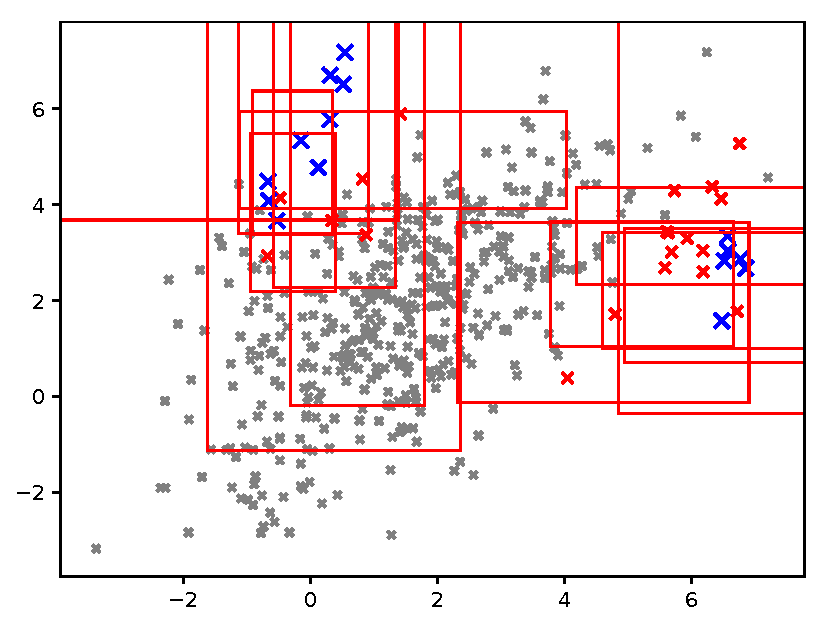
\includegraphics[width=\textwidth]{leaf_trees/query_candidate_regions_ntop5_100_trees_iforest}
		\caption{Isolation Forest}
		\label{fig:iforest_rects}
	\end{subfigure}
	~ %add desired spacing between images, e. g. ~, \quad, \qquad, \hfill etc. 
	%(or a blank line to force the subfigure onto a new line)
	\begin{subfigure}[b]{0.3\textwidth}
		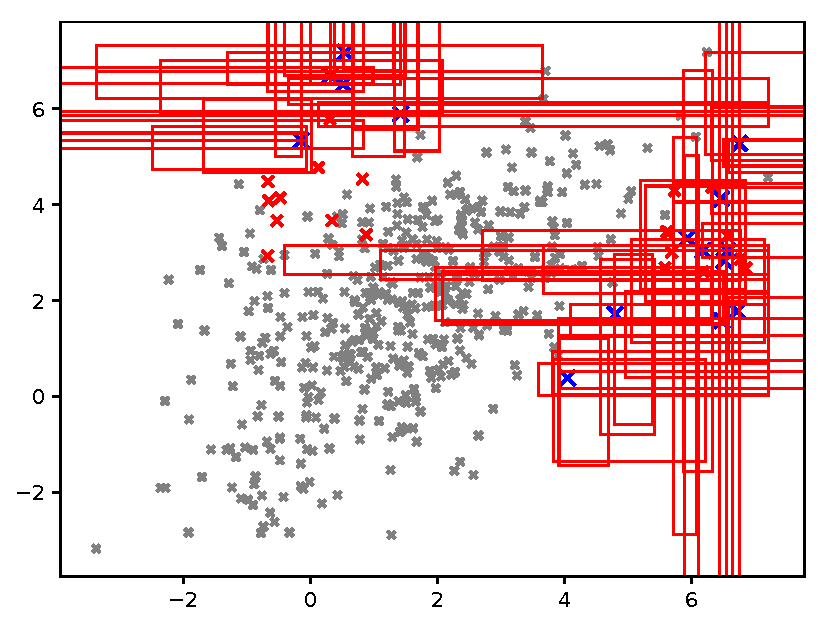
\includegraphics[width=\textwidth]{leaf_trees/query_candidate_regions_ntop5_50_trees_hstrees}
		\caption{HS Trees}
		\label{fig:hstrees_rects}
	\end{subfigure}
	~ %add desired spacing between images, e. g. ~, \quad, \qquad, \hfill etc. 
	%(or a blank line to force the subfigure onto a new line)
	\begin{subfigure}[b]{0.3\textwidth}
		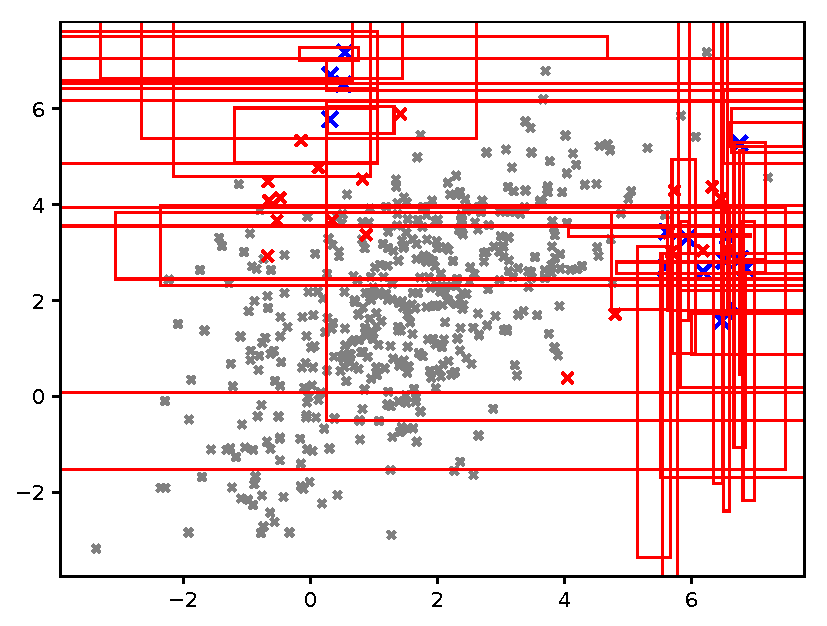
\includegraphics[width=\textwidth]{leaf_trees/query_candidate_regions_ntop5_50_trees_rsforest}
		\caption{RS Forest}
		\label{fig:rsforest_rects}
	\end{subfigure} \\
    \begin{subfigure}[b]{0.3\textwidth}
    	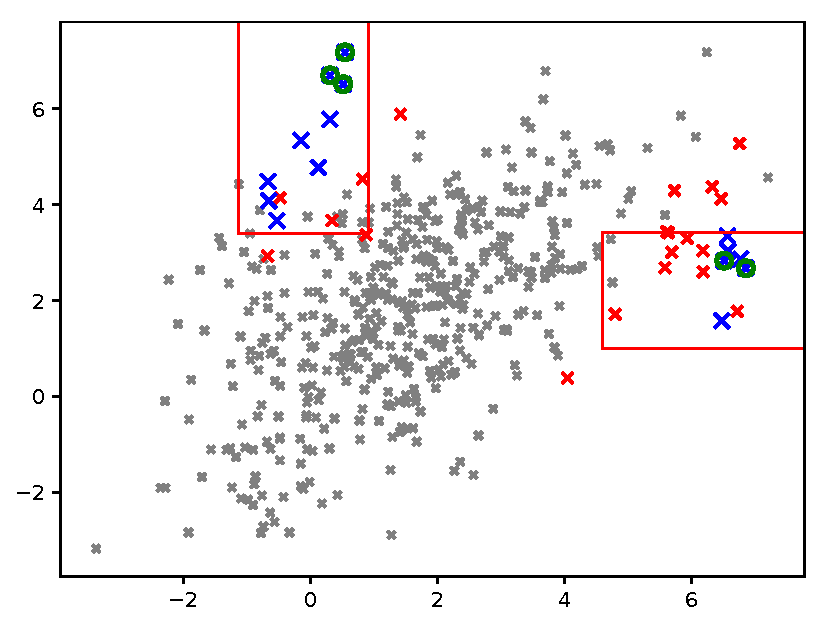
\includegraphics[width=\textwidth]{leaf_trees/query_compact_ntop5_100_trees_aad_iforest}
    	\caption{IForest Compact}
    	\label{fig:iforest_compact_rects}
    \end{subfigure}
    ~ %add desired spacing between images, e. g. ~, \quad, \qquad, \hfill etc. 
    %(or a blank line to force the subfigure onto a new line)
    \begin{subfigure}[b]{0.3\textwidth}
    	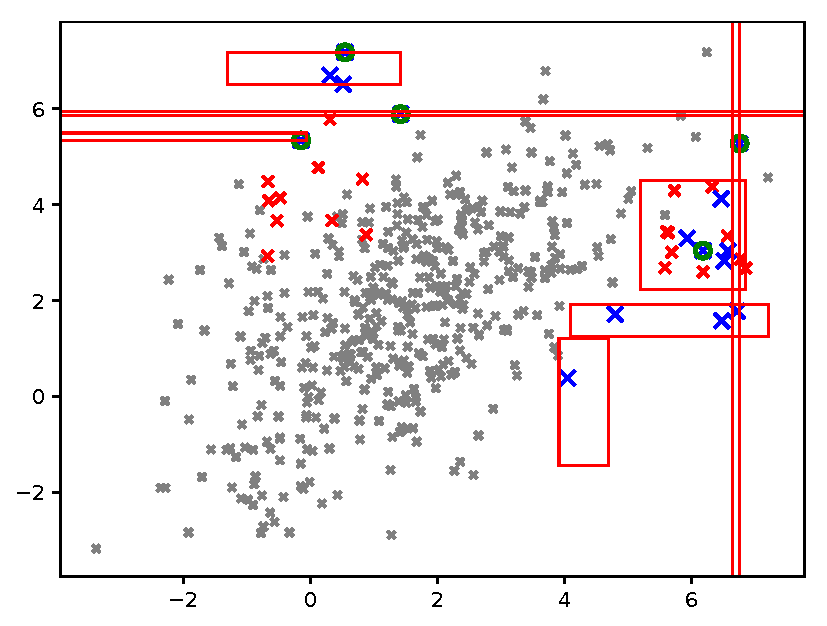
\includegraphics[width=\textwidth]{leaf_trees/query_compact_ntop5_50_trees_aad_hstrees}
    	\caption{HST Compact}
    	\label{fig:hstrees_compact_rects}
    \end{subfigure}
    ~ %add desired spacing between images, e. g. ~, \quad, \qquad, \hfill etc. 
    %(or a blank line to force the subfigure onto a new line)
    \begin{subfigure}[b]{0.3\textwidth}
    	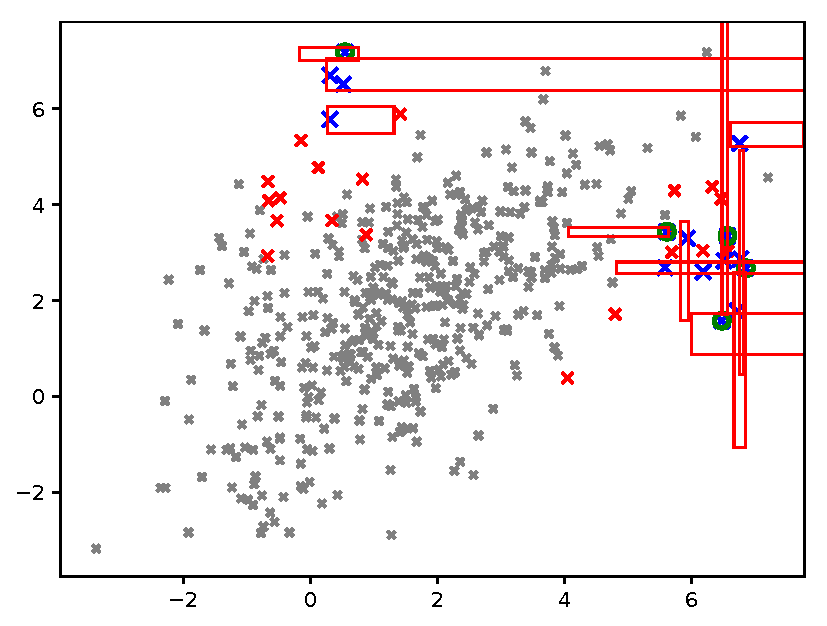
\includegraphics[width=\textwidth]{leaf_trees/query_compact_ntop5_50_trees_aad_rsforest}
    	\caption{RSF Compact}
    	\label{fig:rsforest_compact_rects}
    \end{subfigure}
	\caption{Top subspaces after $35$ feedback iterations ranked by ${\bf w}\circ{\bf d}$ which cover the top ranked $15$ instances. We find the top $5$ most anomalous regions for each of the $15$ instances and the union of all these regions is shown as the \textcolor{red}{red} rectangles (\textbf{top row}). The corresponding compact subspaces which describe the $15$ instances are shown in the \textbf{bottom row}. The points circled in \textcolor{green}{green} (in the bottom row) are the $5$ instances (out of the $15$) selected for query using a diverse querying strategy. The Isolation Forest subspaces tend to be larger and each subspace usually contains more instances. This lets the feedback in Isolation Forest to be shared across more instances than in HS Trees or RS Forest.} \label{fig:tree_diffs}
\end{figure}

\begin{thebibliography}{1}
\bibitem{macha:2017} Meghanath Macha and Leman Akoglu {\em {X-PACS:} eXPlaining Anomalies by Characterizing Subspaces},  2017, http://arxiv.org/abs/1708.05929.
\end{thebibliography}

\end{document}
